\chapter{Implementation}
\graphicspath{{Chapter4/Figs/}{Chapter4/Figs/}}

This chapter goes into the implementation details of building the software-parts for the NIP of IDUN and the key events that occurred during the empirical software engineering process such as the realisation of the novelty and need of a definition for a N/CI. Next to that the author also discusses other key aspects and learnings from building the system.

\section{Timeline}
\label{chapter4-timeline}

Procedures, such as enlisted in the project stages presented in \autoref{chapter3-project-stages}, are a good guide for project implementation, but in the end, such plans run in unexpected ways. As a result, when researching and implementing a non-trivial system such as a N/CI, it requires a high level of agility.

The effective timeline at the time of writing is shown in \autoref{fig:implementation-timeline}. It includes the previously mentioned project stages, but differently structured as initially described. \autoref{tab:special-project-stages} explains why some project stages were completed differently than initially planned.

\begin{figure}[!ht]
  \centering
  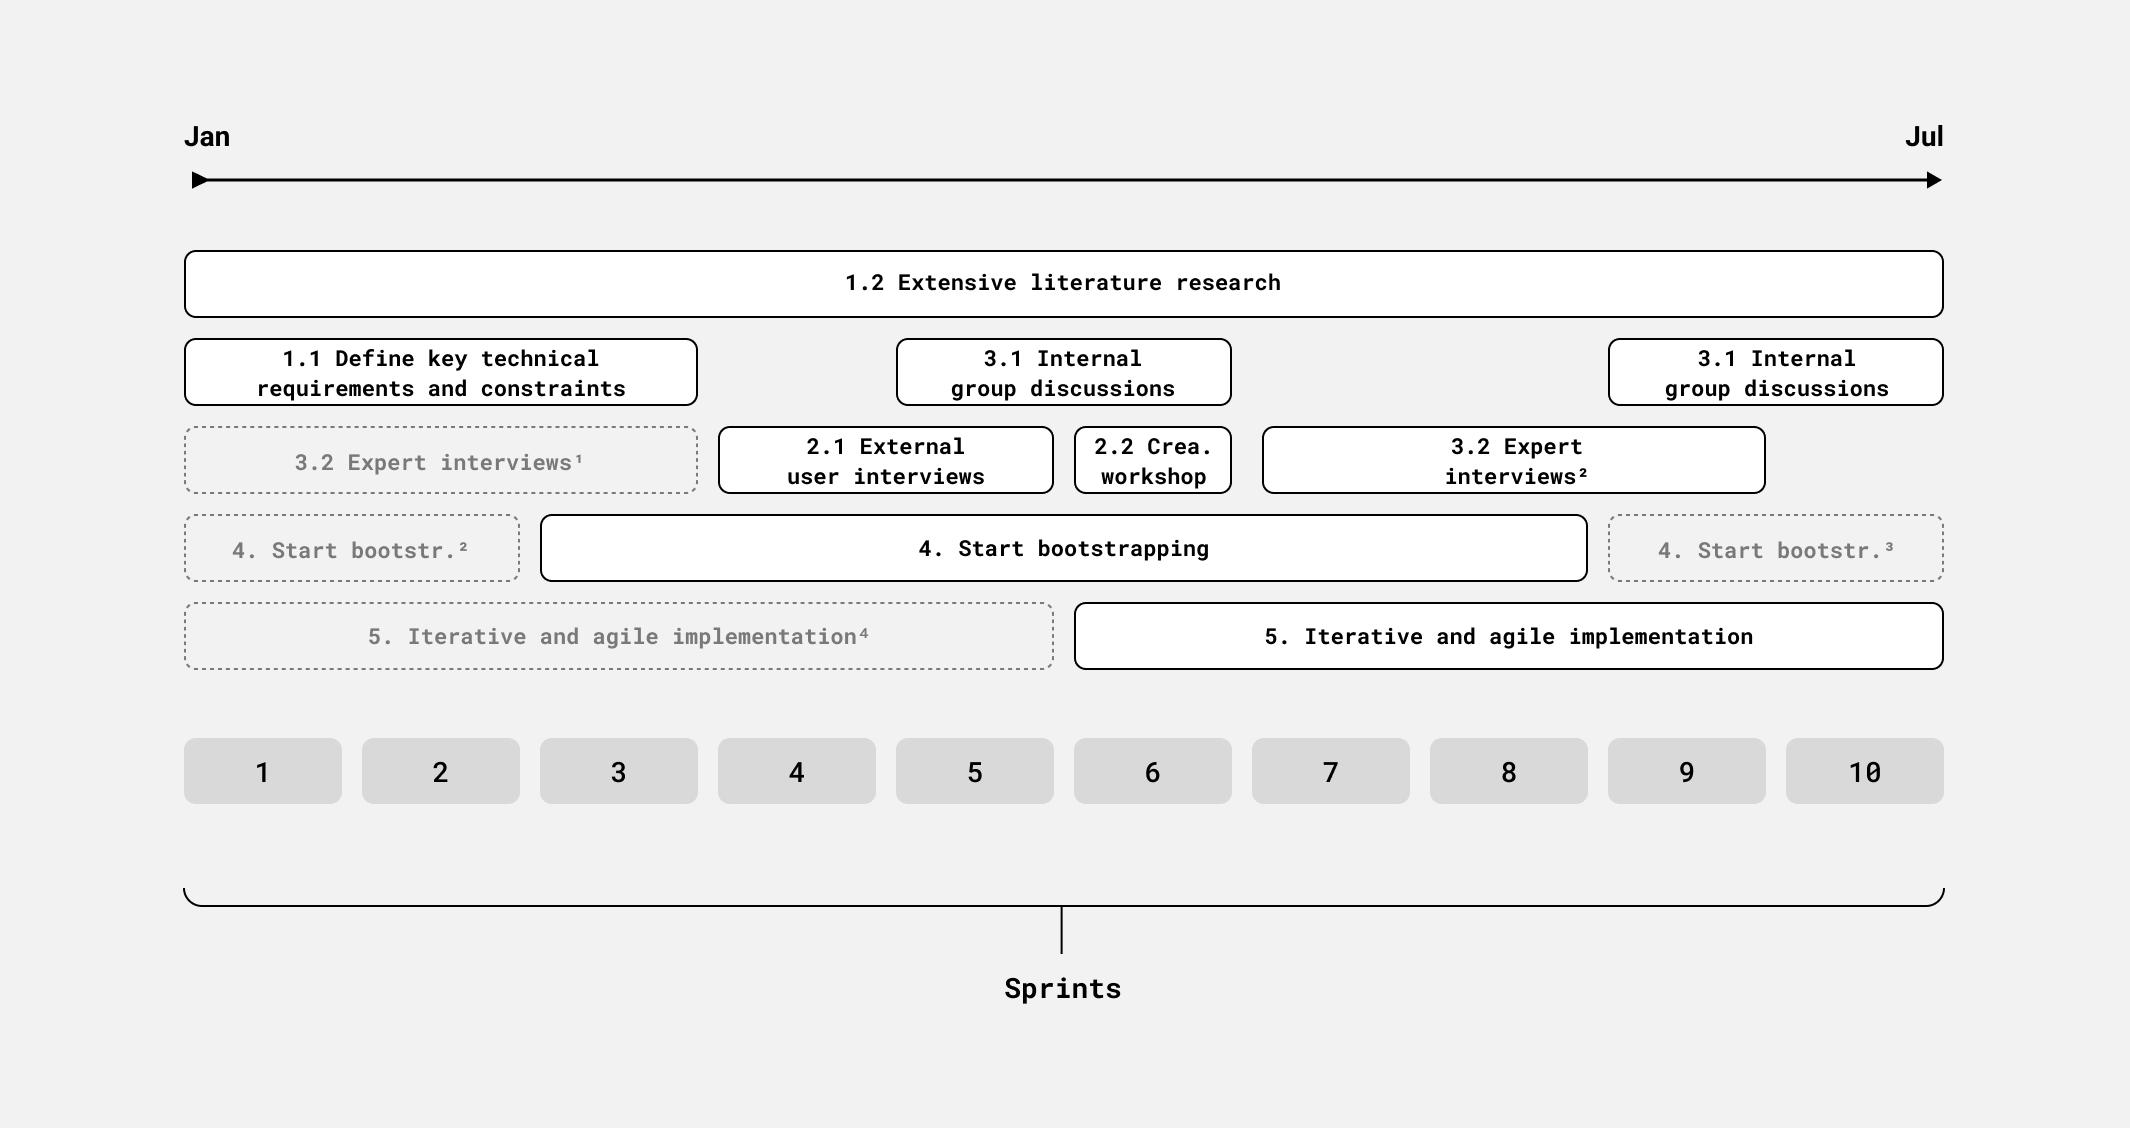
\includegraphics[width=\linewidth]{implementation-timeline.png}
  \caption{Effective timeline of the last ten sprints with project stages in white and specifically planned stages outlined in grey.}
  \label{fig:implementation-timeline}
\end{figure}

\begin{table}[ht]
\centering
\resizebox{\textwidth}{!}{%
\begin{tabular}{
>{\columncolor[HTML]{FFFFFF}}l l}
\cellcolor[HTML]{000000}{\color[HTML]{FFFFFF} Special stage} &
  \cellcolor[HTML]{000000}{\color[HTML]{FFFFFF} Description} \\ \hline
\multicolumn{1}{|l|}{\cellcolor[HTML]{FFFFFF}\textbf{\begin{tabular}[c]{@{}l@{}}[1] 3.2 Expert\\ interviews\end{tabular}}} &
  \multicolumn{1}{l|}{\begin{tabular}[c]{@{}l@{}}The author was able to use the first expert discussions in advance thanks to the help of one\\ of the sales staff's networks. The experts were Nuvibit's experienced enterprise cloud and\\ solution architects. The first topics were strictly technical in nature, focusing on medium-\\ term technological decisions in the context of the company and the timetable.\end{tabular}} \\ \hline
\multicolumn{1}{|l|}{\cellcolor[HTML]{FFFFFF}\textbf{\begin{tabular}[c]{@{}l@{}}[2] 4. Start\\ bootstrapping\end{tabular}}} &
  \multicolumn{1}{l|}{\begin{tabular}[c]{@{}l@{}}This special stage describes the phase in which the author established more organisational\\ structures, such as a professional Scrum or GitHub setup. Furthermore, the time was used\\ to create a more professional AWS organisational setup with various organisational units,\\ as described in the AWS Best Practice Guide \citep{blackham_best_2020}.\end{tabular}} \\ \hline
\multicolumn{1}{|l|}{\cellcolor[HTML]{FFFFFF}\textbf{\begin{tabular}[c]{@{}l@{}}[3] 4. Start\\ bootstrapping\end{tabular}}} &
  \multicolumn{1}{l|}{\begin{tabular}[c]{@{}l@{}}Since the creation of two different Python SDKs (as discussed later in the thesis), more\\ bootstrapping tasks were due at the very end of the given time frame, mostly including\\ the setup of a private PyPi installable Python package and SDK-specific quality\\ assurance pipelines and automations.\end{tabular}} \\ \hline
\multicolumn{1}{|l|}{\cellcolor[HTML]{FFFFFF}\textbf{\begin{tabular}[c]{@{}l@{}}[4] 5. Iterative and\\ agile implementation\end{tabular}}} &
  \multicolumn{1}{l|}{\begin{tabular}[c]{@{}l@{}}Iterative and agile implementation began as soon as needed, without waiting for the design\\ process to be completed (i.e. avoiding a waterfall process). Prior to gaining insights from the \\ design process, time was spent on everything else, such as evaluating technologies, further\\ bootstrapping, first example codebases, or maintaining the old codebase a bit.\end{tabular}} \\ \hline
\end{tabular}%
}
\vspace{10pt}
\caption{Special project stages in the effective schedule as shown in \autoref{fig:implementation-timeline} and their explanation of why they took place there.}
\vspace{-5pt}
\label{tab:special-project-stages}
\end{table}

Several key events occurred during the implementation that shaped the future course of the project and research. This was mostly due to early expert discussions or uncertainties in the requirements as the user-centred design process was still being prepared. These key events are overlaid with the effective project plan as shown in \autoref{fig:implementation-timeline-key-events}. These three green key events are the most influential key events.

\begin{figure}[!ht]
  \centering
  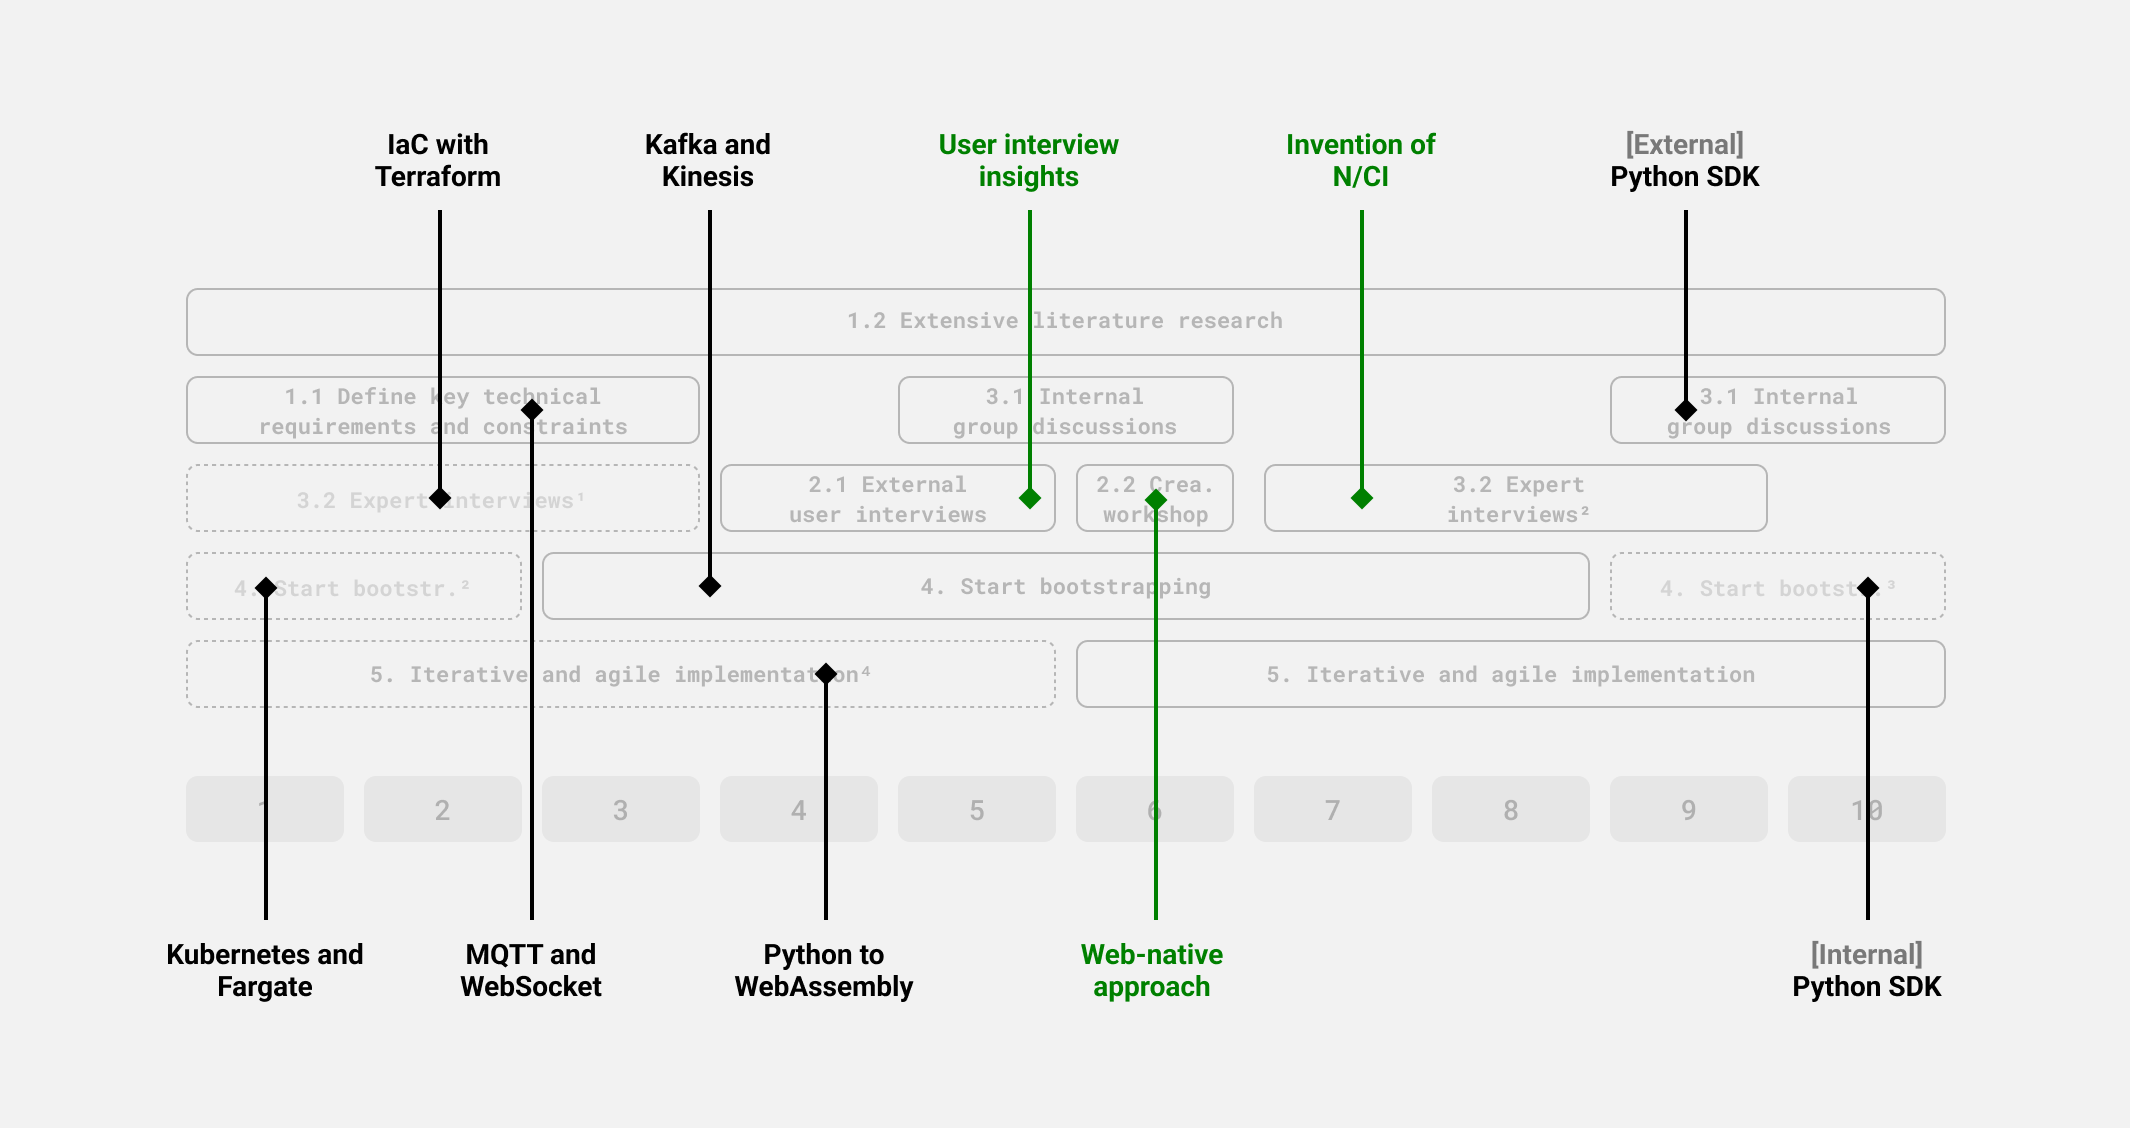
\includegraphics[width=\linewidth]{implementation-timeline-key-events.png}
  \caption{The key events overlaid on the effective project schedule as illustrated in \autoref{fig:implementation-timeline}, with the most influential events coloured green.}
  \label{fig:implementation-timeline-key-events}
\end{figure}

% empirical software engineering done in the case study based on user-centred design process via user interviews or expert interviews and internal group discussions and ongoing literature research.
% MENTION analysis paralysis

\section{Key events}
\label{chapter4-key-events}
% TODO create timeline in Figma

\subsection{User interview insights}
\label{chapter4-user-interview-insights}
% show image of mark and the author doing the user interview

\subsection{Invention of N/CI}
\label{chapter4-invention-of-nci}
% make the connection why the author talked about it in the beginning already

\subsection{Python to WebAssembly}
\label{chapter4-python-to-webassembly}
% mention sprint that we committed to that one
% sushi principle

\subsection{Kubernetes and Fargate}
\label{chapter4-kubernetes-and-aws-fargate}
% quickly explain why microservices
% mention workshop with nuvibit (expert interview)
% mention conversation with jules (expert interview)
% mention centralised system rather than distributed

\subsection{Kafka and Kinesis}
\label{chapter4-kafka-aws-kinesis}
% mention workshop with nuvibit (expert interview)

\subsection{IaC with Terraform}
\label{chapter4-iac-with-terraform}
% mention workshop with nuvibit (expert interview)
% mention workshop with sascha from piavita

\subsection{MQTT and WebSocket}
\label{chapter4-mqtt-and-websocket}
% show image of andy on the whiteboard
% talk about compression and data structure of the EEG data

\subsection{Web-first approach}
\label{chapter4-web-first-approach}
% mention dog feeding and vercel

\subsection{Python SDK}
\label{chapter4-python-sdk}
% mention internal discussions with michel (group discussion)
% mention github limitation of private pypi and registry in general
% mention again the no focus on GUI part from before

\section{Key aspects}
\label{chapter4-key-aspects}

\subsection{Stream-based events}
\label{chapter4-stream-based-events}
% explain event based architecture and the paradigm-shift in building stream based architectures
% talk about concurrency

\subsection{Critical and non-critical}
\label{chapter4-critical-and-non-critical}
% mention the concept from the book and batch processing

\subsection{Hardware-accelerated encryption}
\label{chapter4-hardware-accelerated-encryption}
% mention server-side rendering for privacy
% mention discussion with Andy

\subsection{Per-device auth and opt-in}
\label{chapter4-user-side-opt-in}
% show opt-in wireframes

\subsection{Graph database}
\label{chapter4-graph-database}

\subsection{Feature store and MLOps}
\label{chapter4-feature-store-and-mlops}
% explain MLOps and outlook with Kubeflow
% mention data lakes and data warehouse
% mention internal SDK for feature extraction and experiments
% what is feature extraction and the process
% show image from Wadda

    % However, in practice, it appears that simply making data available quickly—even if it is in a quirky, difficult-to-use, raw format—is often more valuable than trying to decide on the ideal data model up front [54].
